\paragraph{QuizziPedia::Front-End::Views::UserView}
\begin{figure} [ht]
	\centering
	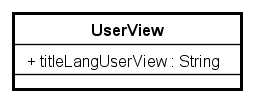
\includegraphics[scale=0.80]{UML/Classi/Front-End/QuizziPedia_Front-end_Views_UserView.png}
	\caption{QuizziPedia::Front-End::Views::UserView}
\end{figure} \FloatBarrier
\begin{itemize}
	\item \textbf{Descrizione}: view contenente le direttive dei dati personali dell'utente, delle sue statistiche relative ai questionari e agli allenamenti effettuati e dei questionari a cui è iscritto;
	\item \textbf{Utilizzo}:  permette ad un utente di visualizzare i propri dati personali e le proprie statistiche e di controllare a quali questionari è iscritto. 
	\item \textbf{Relazioni con altre classi}:
	\begin{itemize}
		\item \textit{IN} \texttt{StatisticsDirective}: directive che permette di visualizzare le statistiche di un utente;
		\item \textit{IN} \texttt{UserDetailsDirective}: directive che permette di visualizzare i dati personali di un utente;
		\item \textit{IN} \texttt{QuestionnaireDetailsDirective}: rappresenta il componente grafico che permette all'utente di visualizzare la lista di questionari che può compilare. Ogni item di questa lista contiene:
		\begin{itemize}
			\item Nome del questionario;
			\item Autore del questionario;
			\item Argomento del questionario;
			\item Parole chiave del questionario;
		\end{itemize}
		Al verificarsi dell'evento click su un item della lista l'utente verrà indirizzato alla view per la compilazione del questionario selezionato;
		\item \textit{IN} \texttt{QuestionnaireDetailsDoneDirective}: rappresenta il componente grafico che permette all'utente di visualizzare la lista di questionari che ha già compilato e di conseguenza vederne le valutazioni. Ogni item di questa lista contiene:
		\begin{itemize}
			\item Nome del questionario;
			\item Autore del questionario;
			\item Argomento del questionario;
			\item Parole chiave del questionario;
			\item Valutazione del questionario.
		\end{itemize}
		\item \textit{IN} \texttt{LangModel}: rappresenta il modello delle informazioni per la giusta traduzione dell'applicazione.
	\end{itemize}
	\item \textbf{Attributi}:
		\begin{itemize}
			\item \texttt{+ titleLangUserView: String} \\ Attributo che viene utilizzato per visualizzare la giusta traduzione del titolo della pagina, in italiano o in inglese.
		\end{itemize}
\end{itemize}